\paragraph{QuizziPedia::Front-End::Controllers::QuestionsController}
\begin{figure} [ht]
	\centering
	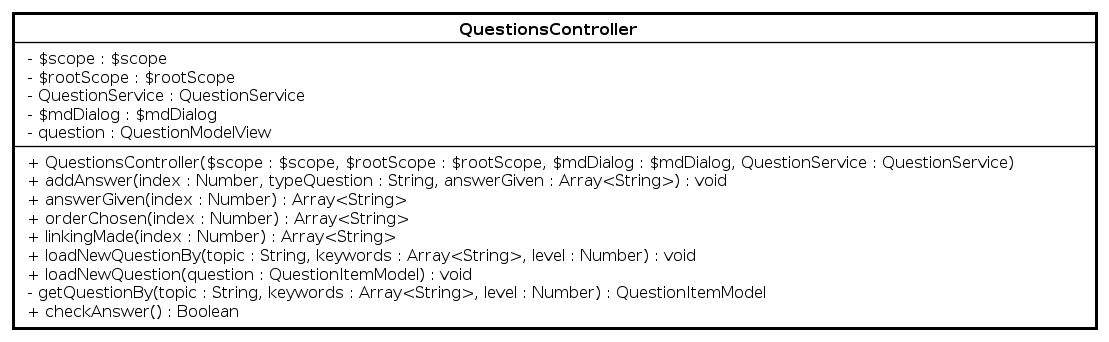
\includegraphics[scale=0.45]{UML/Classi/Front-End/QuizziPedia_Front-end_Controller_QuestionsController.png}
	\caption{QuizziPedia::Front-End::Controllers::QuestionsController}
\end{figure} \FloatBarrier
\begin{itemize}
	\item \textbf{Descrizione}: questa classe permette di gestire il recupero delle domande per far si che possano essere visualizzate nella modalità allenamento e nella compilazione dei questionari;
	\item \textbf{Utilizzo}: fornisce le funzionalità per il recupero delle domande esistenti nel database al fine di poterle visualizzare nella modalità allenamento e nella compilazione dei questionari;
	\item \textbf{Relazione con altre classi}:
	\begin{itemize}
		\item \textit{IN} \texttt{QuestionsModelView}: classe di tipo modelview la cui istanziazione è contenuta all'interno della variabile di ambiente \$scope di \textit{Angular.js\ped{G}}. All'interno di essa sono presenti le variabili e i metodi necessari per il \textit{Two-Way Data-Binding\ped{G}} tra le directive che compongono dinamicamente la vista della domanda e il controller \texttt{QuestionsController};
		\item \textit{IN} \texttt{QuestionServices}: questa classe permette di ottenere domande esistenti e salvare nuove domande;
		\item \textit{IN} \texttt{QuestionItemModel}: rappresenta una domanda. Contiene tutte le informazioni necessarie alla presentazione del contenuto della domanda;
		\item \textit{OUT} \texttt{FillingQuestionnaireController}: questa classe permette di gestire la compilazione del questionario;
		\item \textit{OUT} \texttt{TrainingController}: questa classe permette di gestire la modalità allenamento sottoponendo all'utente le giuste domande adatte al suo livello;
	\end{itemize}
	\item \textbf{Attributi}:
	\begin{itemize}
		\item \texttt{-} \texttt{\$scope: \$scope} \\
		Campo dati contenente un riferimento all’oggetto \$scope creato da \textit{Angular\ped{G}}, viene utilizzato come mezzo di comunicazione tra il controller e la view. Contiene gli oggetti che definiscono il model dell’applicazione;
		\item \texttt{-} \texttt{\$rootScope: \$rootScope} \\
		Campo dati contenente il riferimento all'oggetto globale \$rootScope creato da \textit{Angular\ped{G}}. Viene utilizzato per rendere accessibile a tutti i controller e a tutte le view l'oggetto \texttt{QuestionItemModel}. In questo caso viene utilizzato per inserire in \$rootScope l'oggetto di ritorno della chiamata a \texttt{getQuestion} del service \texttt{QuestionsService};
		\item \texttt{-} \texttt{\$mdDialog: \$mdDialog} \\
		Campo dati contenente un riferimento al servizio della libreria \textit{Material for Angular\ped{G}} che permette di creare delle componenti a popup;
		\item \texttt{-} \texttt{QuestionService: QuestionsService}\\ Permette di ottenere domande esistenti tramite chiamata di metodo specifici;
		\item \texttt{-} \texttt{question: QuestionsModelView}:classe di tipo modelview la cui istanziazione è contenuta all'interno della variabile di ambiente \$scope di \textit{Angular.js\ped{G}}. All'interno di essa sono presenti le variabili e i metodi necessari per il \textit{Two-Way Data-Binding\ped{G}} tra le directive che compongono dinamicamente la vista della domanda e il controller \texttt{QuestionsController}.
	\end{itemize}
	\item \textbf{Metodi}:
	\begin{itemize}
		\item \texttt{+} \texttt{QuestionsController(\$scope: \$scope, \$rootScope: \$rootScope,\$mdDialog: \$mdDialog, QuestionService: QuestionService)}: \\ Metodo costruttore della classe. Interagendo con l'oggetto \texttt{QuestionItemModel} ricevuto si interfaccia con la view andando a visualizzare la giusta directive della tipologia di domanda. \\
		\textbf{Parametri}:
		\begin{itemize}
			\item \texttt{-} \texttt{\$scope: \$scope} \\
			Campo dati contenente un riferimento all’oggetto \$scope creato da \textit{Angular\ped{G}}. Viene utilizzato come mezzo di comunicazione tra il controller e la view. Contiene gli oggetti che definiscono il viewmodel e il model dell’applicazione;
			\item \texttt{-} \texttt{\$rootScope: \$rootScope} \\
			Parametro contenente il riferimento all'oggetto globale \$rootScope creato da \textit{Angular\ped{G}}. Viene utilizzato per rendere accessibile a tutti i controller e a tutte le view l'oggetto \texttt{QuestionItemModel}. In questo caso viene utilizzato per inserire in \$rootScope l'oggetto di ritorno della chiamata a \texttt{getQuestion} del service \texttt{QuestionsService}; 
			\item \texttt{-} \texttt{\$mdDialog: \$mdDialog} \\
			Parametro contenente un riferimento al servizio della libreria \textit{Material for Angular\ped{G}} che permette di creare delle componenti a popup;
			\item \texttt{QuestionService: QuestionService} \\ Parametro che permette di ottenere domande esistenti tramite chiamata di metodo specifici;
		\end{itemize}
		\item \texttt{-} \texttt{getQuestionBy(topic: String, keywords: Array[String], level: Number): QuestionItemModel} \\ Metodo che richiede al back-end una domanda. \\
		\textbf{Parametri}:
		\begin{itemize}
			\item \texttt{topic: String} \\
			Parametro contenente l'argomento della domanda;
			\item \texttt{keywords: Array[String]} \\
			Parametro contenente un\texttt{array} di stringhe che rappresenta le keywords scelte per l'allenamento;
			\item \texttt{level: Number} \\
			Parametro contenente il livello dell'utente.
		\end{itemize}
		\item \texttt{+} \texttt{addAnswer(index: Number, typeQuestion: String, answerGiven: Array[String]): void} \\
		Metodo che gestisce l'evento di selezione delle risposte. \\
		\textbf{Parametri}:
		\begin{itemize}
			\item \texttt{index: Number} \\
			Parametro contenente l'indice della risposta di cui si vuole tenere traccia. Rappresenta anche l'indice dell'\texttt{array objAswer} in cui verrà inserito l'oggetto delle risposte date;
			\item \texttt{typeQuestion: String} \\
			Parametro contenente una stringa la quale indica la tipologia della domanda;
			\item \texttt{answerGiven: Array[String]} \\
			Parametro contenente l'array di risposte date dall'utente aggiornato all'ultima iterazione.
		\end{itemize};
		\item \texttt{+} \texttt{answerGiven(index: Number): Array[String]} \\
		Metodo di supporto che ritorna un \texttt{array} di stringhe contenente le risposte date. Si occupa di recuperare le risposte date nelle domande vero/falso, risposta multipla e ad area cliccabile.\\
		\textbf{Parametri}:
		\begin{itemize}
			\item \texttt{index: Number} \\
			Parametro contenente l'indice della risposta di cui si vuole raccogliere le risposte date. 
		\end{itemize}
		\item \texttt{+} \texttt{orderChosen(index: Number): Array[String]} \\
		Metodo di supporto che ritorna un \texttt{array} di stringhe contenente le risposte date. Si occupa di recuperare le risposte date nelle domande ad ordinamento e di riempimento di spazi.\\
		\textbf{Parametri}:
		\begin{itemize}
			\item \texttt{index: Number} \\
			Parametro contenente l'indice della risposta di cui si vuole raccogliere le risposte date. 
		\end{itemize}
		\item \texttt{+} \texttt{linkingMade(index: Number): Array[String]} \\
		Metodo di supporto che ritorna un \texttt{array} di stringhe contenente le risposte date. Si occupa di recuperare le risposte date nelle domande a collegamento.\\
		\textbf{Parametri}:
		\begin{itemize}
			\item \texttt{index: Number} \\
			Parametro contenente l'indice della risposta di cui si vuole raccogliere le risposte date. 
		\end{itemize}
		\item \texttt{+} \texttt{loadNewQuestionBy(topic: String, keywords: Array[String], level: Number): void} \\
		Metodo che gestisce l'evento per scaricare una nuova domanda in base ai parametri passati. Evoca l'evento per inserire la domanda in \texttt{TrainingModelView}. \\
		\textbf{Parametri}:
		\begin{itemize}
			\item \texttt{topic: String} \\
			Parametro contenente l'argomento della domanda;
			\item \texttt{keywords: Array[String]} \\
			Parametro contenente un\texttt{array} di stringhe che rappresenta le keywords scelte per l'allenamento;
			\item \texttt{level: Number} \\
			Parametro contenente il livello dell'utente.
		\end{itemize}
		\item \texttt{+} \texttt{loadNewQuestion(question: QuestionItemModel): void} \\
		Metodo che gestisce l'evento per visualizzare una nuova domanda. \\
		\textbf{Parametri}:
		\begin{itemize}
			\item \texttt{question: QuestionItemModel} \\
			Parametro contenente un riferimento all'oggetto di tipo \texttt{QuestionItemModel}.
		\end{itemize}
		\item \texttt{+} \texttt{checkAnswer(): boolean} \\ 
		Metodo che controlla che le risposte date siano corrette.
	\end{itemize}
\end{itemize}

